\section{Neuronale Netze}

\subsection{Grundlagen für neuronale Netze}

\begin{frame}{Neuronale Netze}
    \begin{figure}[htp]
        \centering
        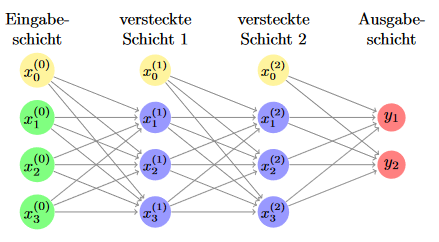
\includegraphics[scale=0.8]{images/neuralnet}
        \caption{Neuronales Netzwerk mit 3 Eingabeneuronen (grün), Bias (gelb), zwei versteckte Schichten
            (blau) und 2 Ausgabeneuronen (rot).}
        \label{neuralNetexample}
    \end{figure}
\end{frame}

\begin{frame}{Neuronale Netze}
    \begin{itemize}
        \item<1-> Ein neuronales Netz besteht aus einer \textbf{Eingabeschicht}, $L-2$ \textbf{versteckte Schichten} und
        einer \textbf{Ausgabeschicht}.
        \item<2-> Jede Schicht $l$ hat $n^{(l)}$ Neuronen sowie ein Bias-Neuron $x_0^{l}$ und die Ausgaben dieser
        Schicht ergibt sich durch
        \[
            x_j^{(l)} = \Psi \left( \sum_{i=1}^{n^{(l)}} \omega_{ij}^{(l)} x_i^{(l-1)} - b_j^{(l)} \right).
        \]
        \item<3-> $\Psi:\mathbb{R} \rightarrow \mathbb{R}$ heißt \textbf{Aktivierungsfunktion} und $\omega_{ij}^{(l)}$
        sind die Gewichte, wobei $b_j^{(l)}:= \omega_{0j}^{(l)}$.
    \end{itemize}
\end{frame}

\begin{frame}{Neuronale Netze: Trainingsprozess}
    \begin{itemize}
        \item<1-> Ziel des Trainingsprozesses ist die Minimierung der Kostenfunktion $\mathcal{C}$.
        \item<2-> Der Trainingsprozess besteht aus \textbf{Forwardpropagation} und
        \textbf{Backwardpropagation}.
        \item<3-> Während der Forwardpropagation werden die Ausgaben der versteckten Schichten Schritt für Schritt berechnet.
        \item<4-> Die Forwardpropagation ist eine Vorbereitung für die Backwardpropagation.
    \end{itemize}
\end{frame}

\begin{frame}{Neuronale Netze: Backwardpropagation}
    \begin{itemize}
        \item<1-> Die Backpropagation ist ein Vorgang, in dem der Gradient der Kostenfunktion $\mathcal{C}$ nach den
        Gewichten $\omega_{ij}^{(l)}$ berechnet wird.
        \item<2-> Der Gradient der Kostenfunktion für die l-te Schicht hat die Form
        \begin{align*}
            \nabla\mathcal{C}=
            \begin{bmatrix}
                \frac{\partial \mathcal{C}}{\partial \omega_{01}^{(l)}} & \dots &
                \frac{\partial \mathcal{C}}{\partial \omega_{n^{(l)}1}^{(l)}} \\
                \vdots & & \vdots \\
                \frac{\partial \mathcal{C}}{\partial \omega_{0n^{(l-1)}}^{(l)}} & \dots &
                \frac{\partial \mathcal{C}}{\partial \omega_{n^{(l)}n^{(l-1)}}^{(l)}} \\
            \end{bmatrix}.
        \end{align*}
        \item<3-> Dabei wird an der Ausgangsschicht $L$ begonnen und rückwärts durch das Netz gearbeitet.
    \end{itemize}
\end{frame}

\begin{frame}{Neuronale Netze: Backwardpropagation}
    \begin{itemize}
        \item<1-> Der Gradient der Kostenfunktion ergibt sich durch
        \begin{align*}
            \frac{\partial \mathcal{C}}{\partial \omega_{ij}^{(l)}} &= \delta_j^{(l)} x_i^{(l-1)}, \\
            \frac{\partial \mathcal{C}}{\partial b_j^{(l)}} &= \delta_j^{(l)} x_{0}^{(l-1)} = -\delta_j^{(l)}.
        \end{align*}
        \item<2-> Der zentrale Teil der Backwardpropagation ist die Berechnung der Deltas
        \begin{align*}
            \delta_i^{(l-1)} = \Psi'(s_i^{(l-1)})\sum\limits_{j=1}^{n^{(l)}} \delta_j^{(l)}\omega_{ij}^{(l)},
            \qquad  i = 1, \dots, n^{(l-1)}
        \end{align*}
        mit den Signalen $s_j^{(l)} = \sum\limits_{i=1}^{n^{(l)}} \omega_{ij}^{(l)} x_i^{(l-1)} - b_j^{(l)}$.
    \end{itemize}
\end{frame}

\begin{frame}{Gradientenverfahren}
    \begin{itemize}
        \item<1-> Nach der Backwardpropagation ist der Gradient der Kostenfunktion bekannt, welcher für ein
        Minimierungsverfahren benötigt wird.
        \item<2-> Ein \textbf{Gradientenverfahren} mit er Lernrate $\mu>0$ hat die Form
        \begin{align*}
            \omega_{ij}^{(l)[k+1]} &= \omega_{ij}^{(l)[k]} - \eta \delta_{j}^{(l)[k]} x_i^{(l-1)[k]}\\
            b_{ij}^{(l)[k+1]} &= b_{ij}^{(l)[k]} + \eta \delta_{j}^{(l)[k]}.
        \end{align*}
    \end{itemize}
\end{frame}

\begin{frame}{Gradientenverfahren: ADAM}
    \begin{itemize}
        \item<1-> Für die numerische Auswertung wird die ADAM (engl. adaptive moment estimation) verwendet.
        \item<2-> Gegeben: $g^{[k]} := \nabla C(\omega^{[k]})$ und die Variablen $\beta_1,\beta_2 \in [0,1)$ sowie die Momente $m^{[0]}=0$,
        $v^{[0]}=0$.
        \item<3-> Die ADAM hat dann die Form
        \[
            \omega_{ij}^{[k+1]}= \omega_{ij}^{[k]} - \eta \frac{\hat{m}^{[k]}}{\sqrt{|\hat{v}^{[k]}|} + \epsilon}
        \]
        mit
        \begin{align*}
            m^{[k]} &= \beta_1 m^{[k-1]} + (1-\beta_1)g^{[k]} \\
            v^{[k]} &= \beta_2 v^{[k-1]} + (1-\beta_2)(g^{[k]})^2
        \end{align*}
        und deren Korrekturen
        \begin{align*}
            \hat{m}^{[k]} = \frac{m^{[k]}}{1-\beta_1^k} \quad \text{ \& } \quad  \hat{v}^{[k]} = \frac{v^{[k]}}{1-\beta_2^k}.
        \end{align*}
    \end{itemize}
\end{frame}

\begin{frame}{Neuronale Netze: verschwindender und explodierender Gradient}
    \begin{itemize}
        \item<1-> Die Berechnung des Gradienten der Kostenfunktion $\nabla \mathcal{C}$ ist fehleranfällig und es können
        zwei Probleme entstehen.
        \item<2-> Das erste Problem wird \textbf{verschwindender Gradient} genannt, wo $\nabla \mathcal{C}\approx0$ gilt.
        \begin{itemize}
            \item<1-> Das Problem entsteht bei bestimmten Aktivierungsfunktionen und eine ungeeignete Gewichtsinitialisierung.
        \end{itemize}
        \item<3-> Das zweite Problem wird \textbf{explodierender Gradient} genannt.
        \begin{itemize}
            \item<1-> Das Problem tritt bei tiefgehenden neuronalen Netze ($L>50$) und bei ungeeigneter
            Gewichtsinitialisierung auf.
        \end{itemize}
    \end{itemize}
\end{frame}

\begin{frame}{Batchtrainig}
    \begin{itemize}
        \item<1-> Die Anzahl der gesamten Trainingsprozesse werden \textbf{Epochen} genannt.
        \item<2-> Ein einzelnes Element der Eingangsdaten $X^{(0)}$ hei0t \textbf{Probe}.
        \item<3-> Die Eingangsdaten werden in \textbf{Batches} $B$ aufgeteilt.
        \item<4-> Vorteil: Es wird an Speicherplatz und Rechenaufwand gespart.
        \item<5-> Dafür wird der Gradient für jede Probe per Backwardpropagation berechnet und der Durchschnitt
        \[
            \widetilde{\nabla C} = \frac{1}{|B|} \sum_{i=1}^{|B|} \nabla C(X^{(0,i)})
        \]
        berechnet.
        \item<6-> Der Durchschnitt wird zur Minimierung der Kostenfunktion $\mathcal{C}$ verwendet.
    \end{itemize}

\end{frame}

\subsection{Prinzip der Lösungspakete}

\begin{frame}{Lösungspakete}
    \begin{itemize}
        \item<1-> Zur Lösung des Anfangswertproblems \eqref{awp-erste-ordnung} gibt es im Allgemeinen keine Trainingsdaten.
        \item<2-> Es wird die Funktion
        \begin{align}
            \label{g-func}
            &G:\mathbb{R}^n \times \mathbb{R}^n \times [t_0, t_f] \times \mathbb{R}^p \rightarrow \mathbb{R}^n \nonumber\\
            &G \left( x, x^{\prime}, t, \theta \right) = x^{\prime} - f(t, x, \theta)
        \end{align}
        definiert, wobei $p \in \mathbb{N}$ die Anzahl der physikalischen Parametern ist.
        \item<3-> Mit den Teilmengen $X_0 \subset \mathbb{R}^n$, $\Theta \subset \mathbb{R}^p$ und $[t_0,t_f] \subset \mathbb{R}$ heißt
        \[
            x(t;x_0, \theta)
        \]
        Lösungspaket für \eqref{g-func}, wobei $t \in [t_0,t_f]$, $x_0 \in X_0$ und $\theta \in \Theta$.
    \end{itemize}
\end{frame}

\begin{frame}{Lösungspakete}
    \begin{itemize}
        \item<1-> Die Approximatiion der Lösung für die Funktion \eqref{g-func} über $(X_0,\Theta)$ ist definiert mit
        \[
            \hat{x}(t;x_0, \theta) = x_0 + a(t) N(t; x_0, \theta; \omega).
        \]
        \begin{itemize}
            \item<1-> Dabei ist $N:\mathbb{R}^{1+n+p} \rightarrow \mathbb{R}^n$ das neuronale Netz mit den Gewichten $\omega$ repräsentiert.
            \item<2-> $a:[t_0,t_f] \rightarrow \mathbb{R}$ hat die Eigenschaft, dass $a(t_0)=0$ ist.
            \item<3-> $a(t) = 1 - e^{t_0-t}$ ist dafür besonders gut geeignet.
        \end{itemize}
    \end{itemize}
\end{frame}

\begin{frame}{Lösungspakete: Kostenfunktion}
    \begin{itemize}
        \item<1-> Es wird eine Funktion $\hat{x}$ gesucht, sodass
        \[
            G(\hat{x}(t_i;x_{0i},\theta_i), \hat{x}^{\prime}(t_i;x_{0i},\theta_i),t_i,\theta_i) \approx 0
        \] gilt.
        \item<2-> Die Kostenfunktion ist gegeben durch
        \begin{align*}
            \mathcal{C} = \frac{1}{|B|} \sum_{(t_i,x_{0i},\theta_i) \in B} \mu(t_i)
            \left\lVert G(\hat{x}(t_i;x_{0i},\theta_i), \hat{x}^{\prime}(t_i;x_{0i},\theta_i),t_i,\theta_i) \right\rVert_2^2.
        \end{align*}
        \begin{itemize}
            \item<1-> Die Batches $B$ bestehen aus Ansammlungen von 3-Tupel $(t_i,x_{0i},\theta_i)$, also
            $B=\{(t_i,x_{0i},\theta_i) \in [t_0,t_f] \times X_0 \times \Theta\}$
            \item<2-> Die Kardinalität $|B|$ wird \textit{Batch Size} genannt.
            \item<3-> $\mu:[t_0,t_f] \rightarrow \mathbb{R}$, $\mu(t) = e^{\lambda (t_0 - t)}$ und $\lambda>0$
        \end{itemize}
    \end{itemize}
\end{frame}

\begin{frame}{Lösungspakete: Fehlerabschätzung}
    \begin{itemize}
        \item<1-> Der lokale Fehler ist definiert durch
        \[
            \tau(t_i;x_{0i}, \theta_i)
            := G \left( \hat{x}(t_i;x_{0i}, \theta_i), \hat{x}^{\prime}(t_i;x_{0i}, \theta_i),t_i;\theta_i \right).
        \]
        \item<2-> Für das Anfangswertproblem \eqref{awp-erste-ordnung} ist der lokale Fehler
        $\tau(t) = \hat{x}^{\prime}(t) - f(t,\hat{x})$ und der globale Fehler $e(t) = \hat{x}(t) - x(t)$.
        \item<3-> Für den globalen Fehler gilt
        \[
            \left\lVert e(t) \right\rVert_2 = \frac{\tau_{t_f}}{L} \left( e^{L(t-t_0)} - 1 \right).
        \]
    \end{itemize}
\end{frame}

\begin{frame}{Intervall-Lernen}
    \begin{itemize}
        \item<1-> Für bestimmte Anfangswertprobleme ist ein Training über das ganze Zeitintervall $[t_0,t_f]$ fehleranfällig.
        \item<2-> In diesen Fällen werden die Batches $B$ angepasst, indem das Zeitinntervall beschränkt wird:
        \[
            B^{\prime}:=  \{(t_i,x_{0i},\theta_i) \in [t_0,t_m] \times X_0 \times \Theta\}.
        \]
        \item<3-> Es gilt $t_m<t_f$ und $m$ ist die Anzahl der bereits trainierten Batches.
        \item<4-> In Anwendung wird
        \[
            t_m = \frac{t_f}{\ln(11)} \ln\left(10 \frac{m}{|B|} + 1 \right), \qquad m = 1, \dots, |B|,
        \]
        und
        \[
            \lambda = \frac{4}{t_m + 5}
        \]
        zur Beschränkung des Zeitintervalls verwendet.
    \end{itemize}
\end{frame}

\begin{frame}{Gewichtsinitialisierung}
    \begin{itemize}
        \item<1-> Es wird im Allgemeinen die \textbf{Xavier- } bzw. \textbf{Glorot-Initialisierung} verwendet, welche die
        Anzahl der Neuronen der $(l-1)$ und $l$-ten Schicht beachtet.
        \item<2-> Für eine lineare Aktivierungsfunktion $\Psi(x)=x$ gilt für die Xavier-Initialisierung der Gewichte
        \[
            \omega_{ij} \sim
            \left[ -\frac{\sqrt {6}}{\sqrt {n^{(l-1)} + n^{(l)}}}, \frac{\sqrt {6}}{\sqrt {n^{(l-1)} + n^{(l)}}} \right].
        \]
        \item<2-> Für die \textbf{ReLU}-Aktivierungsfunktion $\Psi(x)=\tanh(x)$ gilt
        \[
            \omega_{ij} \sim
            \left[ -\frac{\sqrt {6}}{\sqrt {n^{(l-1)} \tanh(2)}}, \frac{\sqrt {6}}{\sqrt {n^{(l-1)} \tanh(2)}} \right].
        \]
    \end{itemize}
\end{frame}

\subsection{Implementierung des neuronalen Netzes}

\begin{frame}{Trainingsablauf}
    \begin{itemize}
        \item<1-> Zuerst wird ein Batch $B_1=\{(t_i,x_{0i},\theta_i)\}$ mit Zufallszahlen aus $[t_0,t_f]$, $X_0$ und $\Theta$
        generiert.
        \begin{itemize}
            \item<1-> Die Anzahl der Tripel wird durch die Batch Size $|B|$ festgelegt.
        \end{itemize}
        \item<2-> Es wird ein neuronales Netz mit $L$ Schichten und $n^{(l)}$, $l=1,\dots,L$ erstellt.
        \item<3-> Die Aktivierungsfunktion wird gesetzt: $\Psi(x)=\tanh(x)$
        \item<4-> Die Gewichte werden mit Xavier-Initialisierung gesetzt.
        \item<5-> Mit Forward-, Backwardpropagation und Gradientenverfahren wird die Kostenfunktion $\mathcal{C}$ für
        jedes Tripel $(t_i,x_{0i},\theta_i)$ minimiert.
        \item<6-> Es wird ein neuer Batch $B_2$ initialisiert.
        \item<7-> Die Gewichte werden für jeden Batch weiterverwendet.
    \end{itemize}
\end{frame}